% Subseção 5.1.1, "Famílias de evidência e respectivos protocolos", mantida fora
% do PDF por decisão do autor em 2026-10-11: a tabela de protocolos e o mapa das
% execuções repetiam o que as seções do Capítulo 6, as notas das tabelas geradas e
% o Capítulo 8 (sec:validade_conclusao) já declaram. As duas regras de leitura
% passaram ao segundo parágrafo da Seção 5.1, e o parágrafo sobre as 60 execuções,
% ao item "Coorte" da Seção 5.2.4.
%
% Para restaurar: descomente o \input em cap_V.tex, reative \usepackage{tikz} em
% main.tex (só o núcleo; as bibliotecas da TikZ não estão no cache offline do
% Tectonic) e volte a apontar para tab:familias_evidencia e fig:mapa_evidencia as
% remissões trocadas nesta data em cap_II, cap_V, cap_VI, cap_VII,
% cap_VII_complementares e cap_VIII.

\subsection{Famílias de evidência e respectivos protocolos}
\label{sec:familias}

Seis famílias de evidência sustentam esta dissertação, cada uma com protocolo próprio, e a Tabela~\ref{tab:familias_evidencia} declara as diferenças. Nas famílias de evidência corrigidas pelo procedimento de Holm~\cite{holm1979simple}, controla-se a taxa de erro por família de hipóteses; nas de hospedeiros e de ativação, o procedimento de Benjamini--Hochberg~\cite{benjamini1995controlling} controla a taxa de falsas descobertas (Seção~\ref{sec:inferencia}), e cada família de evidência conserva a correção da análise em que foi originalmente relatada. A coorte de cada família é o conjunto de execuções que ela usa; a Seção~\ref{sec:estatistica} descreve a da avaliação comparativa principal, e a Figura~\ref{fig:mapa_evidencia} mostra as quatro famílias que reutilizam parte dessa coorte. Duas regras derivam dessas diferenças e valem para todo o texto: contagens de famílias distintas não são somadas, e coortes que se sobrepõem não constituem replicação independente.

\begin{table}[!htb]
    \centering
    \small
    \caption[Protocolo por família de evidência]{Protocolo de cada família de evidência, por questão de pesquisa.}
    \label{tab:familias_evidencia}
    % Linhas agrupadas por questão de pesquisa. Dados e Inferência separam o que a
    % família observa do modo como testa. O reúso de execuções entre famílias fica
    % na Figura~\ref{fig:mapa_evidencia}, e não numa coluna desta tabela.
    \setlength{\tabcolsep}{3pt}
    \begin{tabularx}{\textwidth}{@{}lLlccll@{}}
        \toprule
        & & & \multicolumn{2}{c}{\textbf{Dados}} & \multicolumn{2}{c}{\textbf{Inferência}} \\
        \cmidrule(lr){4-5}\cmidrule(l){6-7}
        \textbf{QP} & \textbf{Família} & \textbf{Papel} & \textbf{Instâncias} & \textbf{Execuções} & \textbf{Pareado por} & \textbf{Correção} \\
        \midrule
        QP1 & \textbf{Comparação principal} & \textbf{Principal} & 51 & 60       & ---            & Holm \\
            & Engenharia                    & Apoio externo      & 3  & 60       & ---            & nenhuma$^{a}$ \\
        \addlinespace
        QP2 & Calibração                    & Apoio              & 12 & 30$^{b}$ & ---            & Holm \\
            & Ablação                       & Apoio              & 51 & 60       & ---            & Holm$^{c}$ \\
        \addlinespace
        QP3 & Hospedeiros                   & Comparativo        & 51 & 30       & execução$^{d}$ & BH \\
        \addlinespace
        QP4 & Ativação do operador          & Diagnóstico        & 51 & 30$^{e}$ & semente        & BH \\
        \addlinespace
        QP5 & Algoritmos comparados         & Contextual         & 51 & 60       & ---            & Holm \\
        \bottomrule
    \end{tabularx}
    \par\smallskip
    \parbox{\textwidth}{\footnotesize
    QP: questão de pesquisa. Execuções: número de execuções por algoritmo e instância. Calibração e ablação formam uma família, com uma linha por estudo. Sem pareamento (---), teste de soma de postos de Wilcoxon (Mann--Whitney) bicaudal; com pareamento, teste de postos sinalizados de Wilcoxon. BH: Benjamini--Hochberg. Todas as famílias reportam IGD e HV; na de ativação, o HV é a métrica primária declarada, porque os rótulos de instância derivam da comparação em IGD da coorte da comparação principal.\\
    $^{a}$Com Holm entre os três problemas, nenhuma decisão muda. $^{b}$Com 50.000 avaliações por execução; o braço histórico tem 60 execuções. $^{c}$A fase fatorial usou o teste de Friedman. $^{d}$Nos pares NSGA; no par IVF/SPEA2, execuções alinhadas por ordem. $^{e}$Teste do controlador; os observáveis da dinâmica comparam as classes de instância por Mann--Whitney, e os rótulos vêm das 60 execuções da coorte da comparação principal.}
\end{table}

\begin{figure}[!htb]
    \centering
    % Mapa das famílias de evidência: à esquerda, a coorte da comparação principal;
    % no centro, cada família com o seu teste e a sua correção; à direita, as
    % execuções geradas para a família. Coordenadas absolutas, sem bibliotecas da
    % TikZ, porque o build roda com o cache offline do Tectonic.
    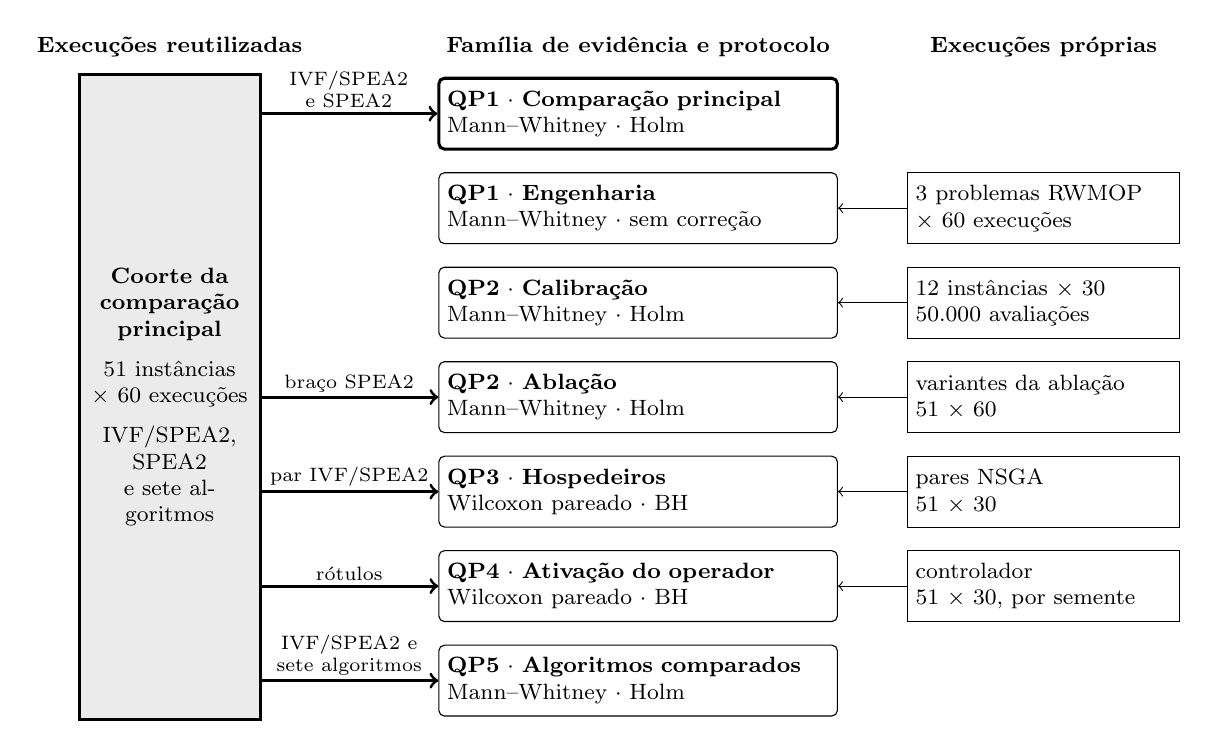
\begin{tikzpicture}[x=1cm, y=1cm, font=\footnotesize,
        fam/.style={draw, rounded corners=2pt, text width=4.85cm, align=left, inner sep=3pt, minimum height=0.9cm},
        dat/.style={draw, text width=3.25cm, align=left, inner sep=3pt, minimum height=0.9cm},
        reuso/.style={->, line width=1.1pt},
        propria/.style={->, line width=0.4pt},
        rotulo/.style={font=\scriptsize, above, align=center, inner sep=1.5pt}]
        \fill[black!8] (0,0.5) rectangle (2.3,-7.7);
        \draw[line width=1.1pt] (0,0.5) rectangle (2.3,-7.7);
        \node[text width=2.0cm, align=center] at (1.15,-3.6) {\textbf{Coorte da comparação principal}\\[5pt]51 instâncias\\$\times$ 60 execuções\\[5pt]IVF/SPEA2, SPEA2\\e sete algoritmos};
        \node[fam, line width=1.1pt] (f1) at (7.1,0) {\textbf{QP1 $\cdot$ Comparação principal}\\Mann--Whitney $\cdot$ Holm};
        \draw[reuso] (2.3,0) -- node[rotulo] {IVF/SPEA2\\e SPEA2} (f1.west);
        \node[fam] (f2) at (7.1,-1.2) {\textbf{QP1 $\cdot$ Engenharia}\\Mann--Whitney $\cdot$ sem correção};
        \node[dat] (df2) at (12.25,-1.2) {3 problemas RWMOP\\$\times$ 60 execuções};
        \draw[propria] (df2.west) -- (f2.east);
        \node[fam] (f3) at (7.1,-2.4) {\textbf{QP2 $\cdot$ Calibração}\\Mann--Whitney $\cdot$ Holm};
        \node[dat] (df3) at (12.25,-2.4) {12 instâncias $\times$ 30\\50.000 avaliações};
        \draw[propria] (df3.west) -- (f3.east);
        \node[fam] (f4) at (7.1,-3.6) {\textbf{QP2 $\cdot$ Ablação}\\Mann--Whitney $\cdot$ Holm};
        \draw[reuso] (2.3,-3.6) -- node[rotulo] {braço SPEA2} (f4.west);
        \node[dat] (df4) at (12.25,-3.6) {variantes da ablação\\51 $\times$ 60};
        \draw[propria] (df4.west) -- (f4.east);
        \node[fam] (f5) at (7.1,-4.8) {\textbf{QP3 $\cdot$ Hospedeiros}\\Wilcoxon pareado $\cdot$ BH};
        \draw[reuso] (2.3,-4.8) -- node[rotulo] {par IVF/SPEA2} (f5.west);
        \node[dat] (df5) at (12.25,-4.8) {pares NSGA\\51 $\times$ 30};
        \draw[propria] (df5.west) -- (f5.east);
        \node[fam] (f6) at (7.1,-6.0) {\textbf{QP4 $\cdot$ Ativação do operador}\\Wilcoxon pareado $\cdot$ BH};
        \draw[reuso] (2.3,-6.0) -- node[rotulo] {rótulos} (f6.west);
        \node[dat] (df6) at (12.25,-6.0) {controlador\\51 $\times$ 30, por semente};
        \draw[propria] (df6.west) -- (f6.east);
        \node[fam] (f7) at (7.1,-7.2) {\textbf{QP5 $\cdot$ Algoritmos comparados}\\Mann--Whitney $\cdot$ Holm};
        \draw[reuso] (2.3,-7.2) -- node[rotulo] {IVF/SPEA2 e\\sete algoritmos} (f7.west);
        \node[font=\footnotesize\bfseries] at (1.15,0.85) {Execuções reutilizadas};
        \node[font=\footnotesize\bfseries] at (7.1,0.85) {Família de evidência e protocolo};
        \node[font=\footnotesize\bfseries] at (12.25,0.85) {Execuções próprias};
    \end{tikzpicture}
    \caption[Execuções usadas por família de evidência]{Execuções usadas por família de evidência. Setas grossas: execuções da coorte da comparação principal reutilizadas pela família, cujas contagens, por isso, não são observações independentes das da comparação principal. Setas finas: execuções geradas para a família.}
    \label{fig:mapa_evidencia}
\end{figure}

